\section{Cinematica}
%%
\subsection{Moto rettilineo}
\begin{gather*}
\textbf{Variazione di velocità: } \Delta v = v - v_0 \\
\textbf{Tempo trascorso: } \Delta t = t - t_0 \\
\textbf{Distanza percorsa: } \Delta s = \left| s - s_0 \right|
\end{gather*}
\subsection{Moto accelerato}
\textbf{Nota bene: } questo sistema si usa spesso e volentieri per il moto uniforme
\begin{gather*}
\begin{cases}
    v = v_0 + a_t \\
    s = s_0 + v_0 t + \frac{1}{2} a t^2
\end{cases}
\\
\textbf{Accelerazione:} \\
\begin{cases}
 a = g = 9.81 m/s^2 & \text{Caduta libera} \\
 a = -g = - 9.81m/s^2 & \text{Lancio in alto}
\end{cases}
\\
\textbf{Velocità: } v = v_0 + a t \\
\textbf{Tempo: } t = \frac{v - v_0}{a} \\
\textbf{Accelerazione: } a = \frac{v - v_0}{t} \\
\textbf{Accelerazione: } a = \frac{2 (s - s_0 - v_0 t)}{t^2} \\
\textbf{Velocità(senza t): } v = \sqrt{v_0^2 + 2 a (s - s_0)} \\
\textbf{Posizione: } s = s_0 + v_0 t + \frac{1}{2} a t^2 \\
\textbf{Posizione(senza a): } s = s_0 + \frac{v + v_0}{2} t \\
\textbf{Velocità(senza a): } v = \frac{2 (s - s_0)}{t} - v_0
\end{gather*}
%%%
\subsection{Moto parabolico}
\textbf{Nota bene: } l'accelerazione($g$)è negativa quando si presume di partire dal basso verso l'alto, perché la gravita agisce contro il movimento verticale. \\ Al contrario, se ci troviamo in un movimento che parte dall'alto verso il basso, l'accelerazione($g$)sarà positiva!
\begin{gather*}
\textbf{Equazione parabola: } \\ \begin{cases}
    x = x_0 + v_{0x} t \\
    y = y_0 + v_{0y} t - \frac{1}{2} g t^2
\end{cases}
\\
\textbf{Equazione parabola: } \\ y = \frac{v_x}{v_y} x - \frac{1}{2} \frac{g}{v_x^2} x^2 \\
\textbf{Velocità iniziale: } v_0 = \sqrt{v_x^2 + v_y^2} \\
\textbf{Velocità iniziale: } \\ \begin{cases}
    v_{0x} = v_0 \cos \alpha  = v_y \frac{\cos \alpha}{\sin \alpha} \\
    v_{0y} = v_0 \sin \alpha = v_x \frac{\sin \alpha }{\cos \alpha}
\end{cases}
\\
\textbf{Velocità(tempo t): } \begin{cases}
    v_x = v_0 \cos \alpha \\
    v_y = v_0 \sin \alpha - a t
\end{cases}
\\
\textbf{Vertice: } \begin{cases}
    x_v = \frac{v_x v_y}{g} = \frac{v_0^2 \sin (2\alpha)}{g} \\
    y_v = \frac{v_y^2}{2g}
\end{cases}
\\
\textbf{Gittata: } \frac{v_x v_y}{\frac{1}{2}g} = \frac{v_0^2 \sin (2 \alpha)}{\frac{1}{2}g} \\
\textbf{Tempo di volo: } t = \frac{v_0 \sin \alpha}{2g} \\
\textbf{Altezza massima: } y = \frac{v_0^2 \sin (2 \alpha)}{2g}
\end{gather*}

%%%
\subsection{Moto circolare}
\begin{center}
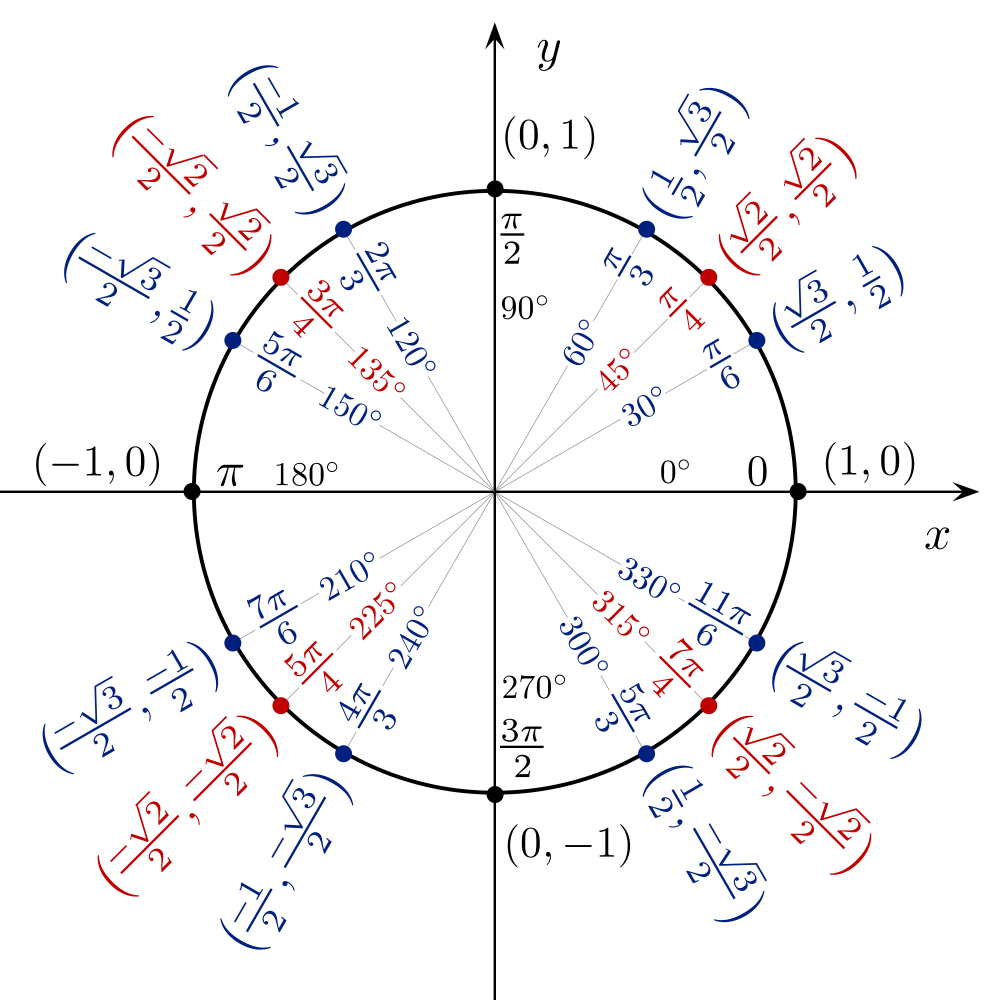
\includegraphics[width=0.8\linewidth]{Cinematica/circonferenza-goniometrica.png}
\end{center}
%%%%
\begin{center}
\begin{tabular}{ c c c }
    Grandezze & Lineari & Angolari \\
    Posizione & $s$ & $\theta$ \\
    Velocità & $v$ & $\omega$ \\
    Accelerazione & $a$ & $\alpha$ \\
\end{tabular}
\end{center}
\textbf{Nota bene: } come la tabella sopra ci indica, c'è una corrispondenza tra grandezze lineari e grandezza angolari. \\ Ciò significa che possiamo immaginare il punto che si muove sulla circonferenza come se si muovesse su una retta(la circonferenza \textit{spiaccicata}), e di conseguenza utilizzare le formule del moto rettilineo per trovarne la posizione!
\begin{gather*}
    \textbf{Velocità: } v = v_0 + a t \\
    \textbf{Tempo: } t = \frac{v - v_0}{a} \\
    \textbf{Accelerazione: } a = \frac{v - v_0}{t} \\
    \textbf{Posizione: } s = s_0 + v_0 t + \frac{1}{2} a t
\end{gather*}
\subsubsection{Moto circolare uniforme}
\textbf{Nota bene: } La velocità tangenziale($v$) indica quanto velocemente il punto si sposta sulla circonferenza($r$); \\
La velocità angolare($\Omega$) indica quanto velocemente cambia l'angolo($\theta$) che il punto forma
\begin{gather*}
 \textbf{Velocità: } v = \frac{\Delta s}{\Delta t} = \frac{2 \pi r}{T} = \omega r = \sqrt{a_c r} \\
\textbf{Raggio: } r = \frac{v T}{2 \pi} = \frac{v}{\omega} = \frac{v^2}{a_c} = \frac{a_c}{\omega^2} \\
\textbf{Periodo: } T = \frac{2 \pi r}{v} = \frac{2 \pi}{\omega} \\
\textbf{Velocità angolare: } \omega = \frac{v}{r} = \frac{2 \pi}{T} = \sqrt{\frac{a_c}{r}} \\
\textbf{Accelerazione centripeta: } a_c = \frac{v^2}{r} = \omega^2 r \\
\textbf{Posizione angolare: } \theta = \frac{s - s_0}{r} \\
\textbf{Legge oraria} \\
\textbf{Posizione angolare: } \theta(t) = \theta_0 + \omega t \\
\textbf{Velocità angolare: } \omega = \frac{\theta - \theta_i}{t - t_i}
\end{gather*}
%%%%
\subsubsection{Moto circolare uniformemente accelerato(MCUA)}
\textbf{Nota bene: } L'accelerazione centripeta($\vec{a}_c$) permette al punto di mantenere la propria traiettoria sulla circonferenza. Cambia il verso, ma non il modulo della velocità($\vec{v}$) \\
L'accelerazione tangenziale($\vec{a}_T$, perpendicolare a $\vec{a}_c$) invece fa variare il modulo della velocità($\vec{v}$), è \textbf{costante}. \\
L'accelerazione totale($\vec{a}_{tot}$) è la risultante delle accelerazioni precedenti \\
\begin{gather*}
\textbf{Accelerazione totale: } \vec{a}_{tot} = \vec{a}_T + \vec{a}_c \\
\textbf{Accelerazione totale: } a_{tot} = \sqrt{a_T^2 + a_c^2} \\
\textbf{Accelerazione angolare: } \alpha = \frac{d \omega}{d t} = \frac{\omega - \omega_0}{t - t_0} \\
\textbf{Accelerazione tangenziale: } a_T = \alpha \cdot r \\
\textbf{Legge oraria} \\
\begin{cases}
    \theta = \theta_0 + \omega_0 t + \frac{1}{2} \alpha t^2 & \text{Posizione angolare} \\
    \omega = \omega_0 + \alpha t & \text{Velocità angolare}
\end{cases} \\
\textbf{Velocità angolare(senza t): } \\ \omega^2 = \omega_0^2 + 2 \alpha(\theta - \theta_0)
\end{gather*}
\subsubsection{Esempio}
\textbf{Nota bene: } per risolvere un problema del tipo: punto materiale con MCUA con $r = 1m$, $s_1 = 0.4m$, $t_1 = 2s$, $t_2 = 4s$, e $v_0 = 0.1 \frac{m}{s}$ dove chiede modulo dell'accelerazione totale al tempo $t_2$(quindi $a_{tot(2)} = \sqrt{a_T^2 + a_{c(2)}^2}$) possiamo impostare il seguente sistema:
\begin{gather*}
    \begin{cases}
        a_{tot(2)} = \sqrt{a_T^2 + a_{c(2)}^2} \\
        a_T = \frac{2(s - s_0 - v_0 t)}{t^2} \\
        a_{c(2)} = \frac{v_2^2}{r} \\ 
        v_{2} = v_0 + a_T \cdot t_2
    \end{cases}
\end{gather*}